\chapter{Kinematics}
\label{chap:kinematics}

\section{Geometry}
\label{sec:Geometry}

The geometry of the leg was first found in the study in 2006 \cite{Yu2006} that investigated a hybrid machine system based on a 5-bar linkage design. This study derived a set of complex kinematic equations to solve for the end effector position given the motor angles. This robot was more of a study in kinematic derivation, and although the same geometry was used, complex kinematic equations were derived that would be difficult to implement on a micro-controller system. The kinematic equations also needed further mapping to the polar coordinate system used in Baleka.

In 2015 a single legged jumping robot was developed in \cite{Duperret} that used the same geometric leg topology - the Baleka design was based off of this robot and the kinematic equations derived in this study were used to implement the virtual model control system for Baleka.

In 2016 a similar leg topology was used in \cite{Kalouche2016} with a three motor 3 DOF geometric design. The virtual model control implemented in this study was adapted and improved for use on Baleka.

The leg linkage length choices that were originally implemented by Ben Bingham based off the design in \cite{Duperret} were validated using a kinematic workspace simulation in this study in \cref{sec:Simulation-Kinematics}. The leg linkage lengths of $l_1 = 0.15\ m$ and $l_2 = 0.3\ m$ were chosen.

The foot of Baleka will be referred to often in the design. The foot is the intersection between the lower linkages, $l_2$, and is the end effector of the robot.

In the design of leg dynamics, a radial set-point is often spoken of rather than a radial position or command. This set-point is a radial distance in the virtual model, further developed in \cref{chap:Dynamic Modelling}, that indicates the length of the leg spring-damper system at rest, measured from the midpoint between the two motors to the foot. A radial offset indicates the difference between the virtual model radial set-point and the actual end effector radial position. With a virtual model control system, you don't command a position, but rather define the virtual model set-points for a certain natural response.

When facing the leg, the rotational set-point of the leg might be specifically spoken of as either the angular set-point ($\theta$) or the arc-length set-point ($s$), measured anti-clockwise from the negative y-axis. 

Both of the motor angles, $\phi_1$ and $\phi_2$, are measured from the positive y-axis to the first linkage $l_1$, as shown in \cref{fig:Geometric view of leg} - this measurement is calibrated by placing the end effector vertically down with linkage pairs parallel and setting the encoder positions to zero counts. The microcontroller then calculates the appropriate motor angles using the motor driver feedback count values.

\begin{figure}
\centering
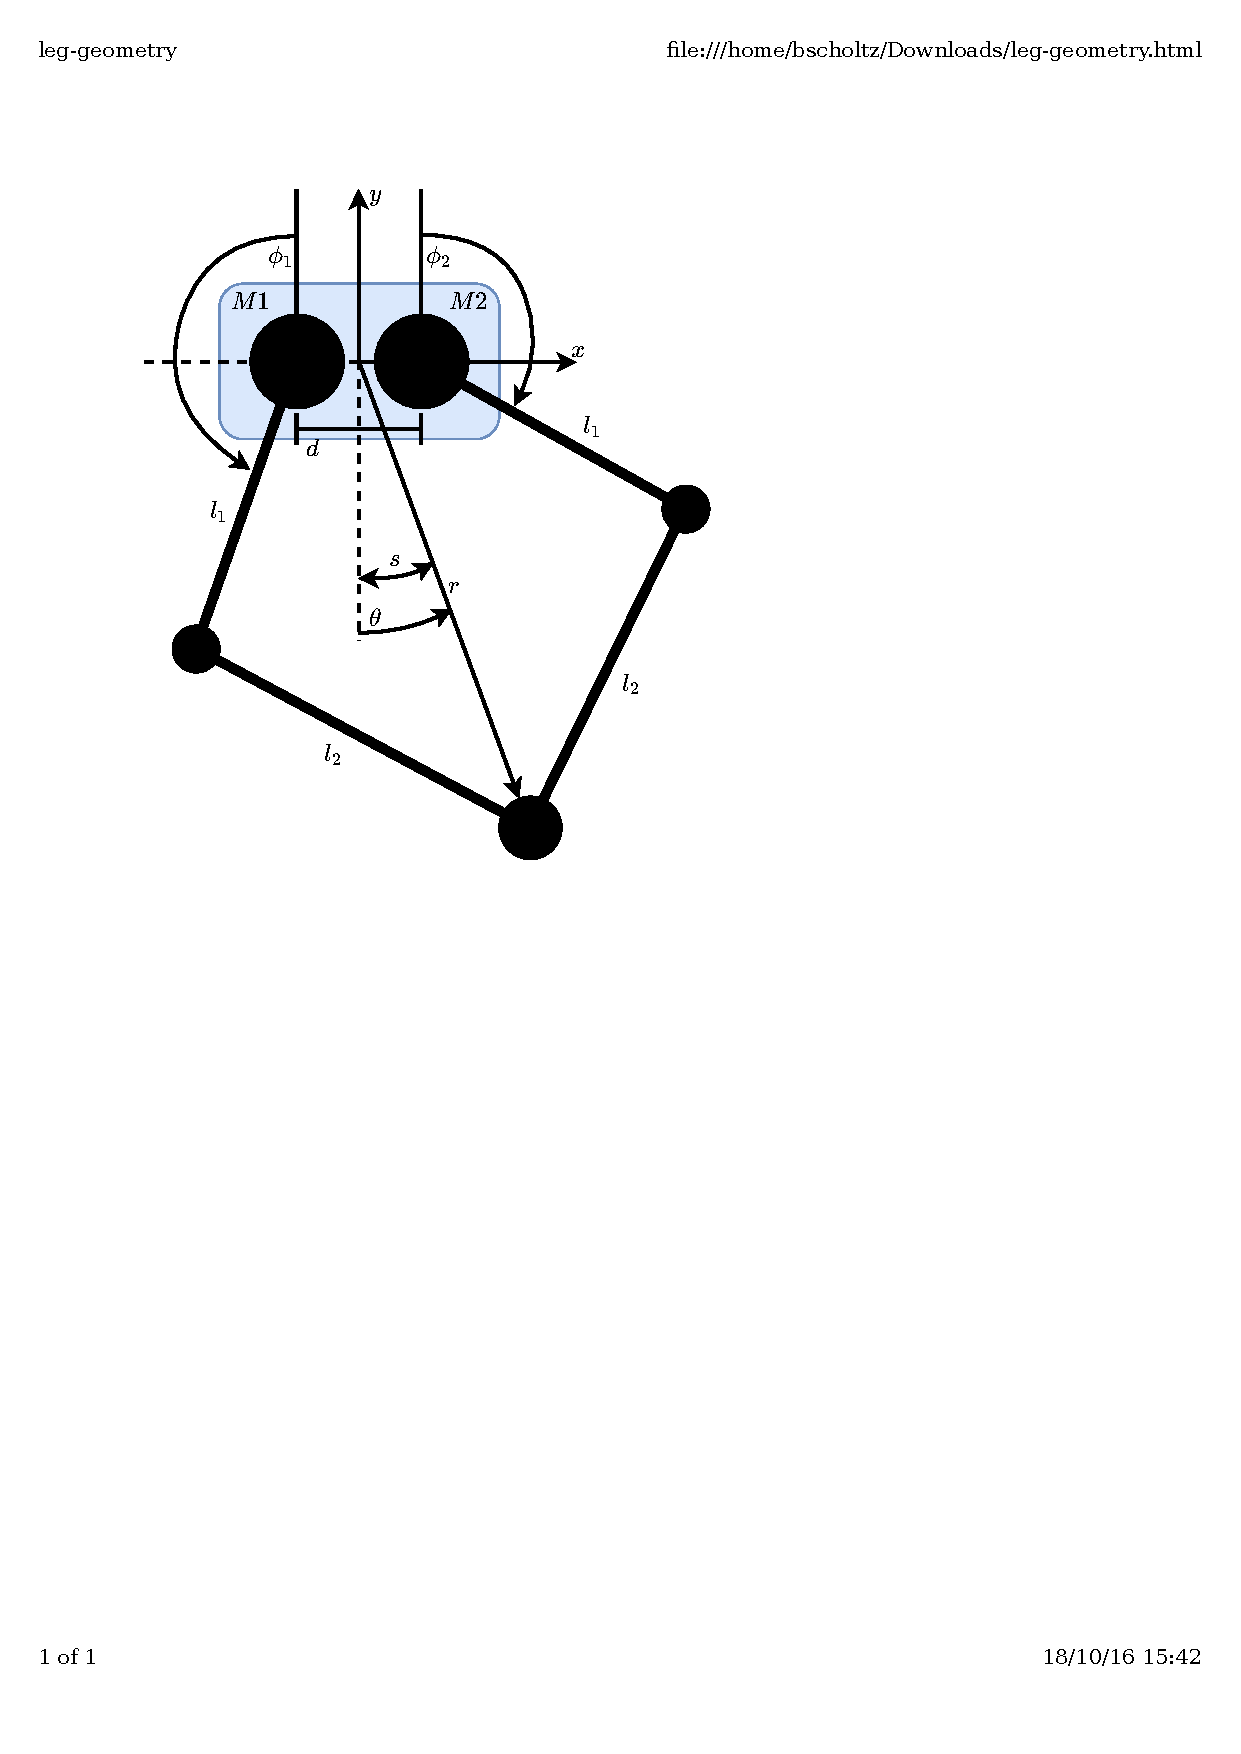
\includegraphics[clip, trim=2cm 15cm 7cm 2cm, page = 1, width=0.8\textwidth]{images/geometry/leg-geometry} 
\caption{Geometric view of leg.}
\label{fig:Geometric view of leg}
\end{figure}

\section{Kinematic Equations}
\label{sec:Kinematic Equations}
The geometry of the leg is fairly complex and the derivation of the kinematic equations equally so. J.M. Duperret and D.E. Koditschek derived the kinematic equations \cref{eq:forward-kinematics,eq:reverse-kinematics} in the study \cite{Duperret}. 

In this study the assumption was made that the distance $d$, as seen in \cref{fig:Geometric view of leg}, is zero. This simplifies the derivation of forward and reverse kinematic equations of the leg design by making the leg a 4-bar linkage. These kinematic equations are more easily calculated on board a microcontroller\cite{Duperret}, leaving more processing power for other control tasks if needed. 

The ease of calculation makes the loss in accuracy acceptable - in practise the simplified kinematic equations worked well with an insignificant calculation time made possible by the STM32F4's on-board floating point unit, and insignificant kinematic distortion.

\subsubsection{Forward Kinematic Map}
\begin{equation} \label{eq:forward-kinematics}
f(\phi_1, \phi_2) = \left(\begin{array}{c} \sqrt{{\mathrm{l_2}}^2 - {\mathrm{l_1}}^2\, {\sin\!\left(\frac{\mathrm{\phi_1}}{2} + \frac{\mathrm{\phi_2}}{2}\right)}^2} - \mathrm{l_1}\, \cos\!\left(\frac{\mathrm{\phi_1}}{2} + \frac{\mathrm{\phi_2}}{2}\right)\\
\frac{\mathrm{\phi_1}}{2} - \frac{\mathrm{\phi_2}}{2} \end{array}\right)
\end{equation}

\subsubsection{Inverse Kinematic Map}
\begin{equation} \label{eq:reverse-kinematics}
g(r, \theta) = \left(\begin{array}{c} \pi - acos(\frac{r^2 + l_1^2 - l_2^2}{2rl_1}) + \theta \\
\pi - acos(\frac{r^2 + l_1^2 - l_2^2}{2rl_1}) - \theta  \end{array}\right)
\end{equation}

\section{The Jacobian}
\label{sec:The Jacobian}
The forward kinematic Jacobian is formed by taking partial derivatives of the forward kinematic equation \cref{eq:forward-kinematics} as shown in \cref{eq:jacobian}. In some cases the inverse kinematic Jacobian will be used to implement simulations.

It is used as a mapping from the joint angles $\phi_1$ and $\phi_2$ to the end effector generalized coordinates $r$ and $\theta$. The Jacobian can be applied in robotic kinematic control to determine joint velocities and forces to achieve a desired force or velocity at the end effector, in this case the leg foot.

\subsubsection{Forward Kinematic Jacobian}
\begin{equation} \label{eq:jacobian}
J(\phi_1,\phi_2) = \left[ \frac{\partial \textbf{f}}{\partial \textbf{X}} \right] 
\end{equation}
where \textbf{X} = [$\phi_1$ $\phi_2$] and \textbf{f} = $f(\phi_1, \phi_2)$.

\subsubsection{Inverse Kinematic Jacobian}
\begin{equation} 
J(r,\theta) = \left[ \frac{\partial \textbf{f}}{\partial \textbf{X}} \right] 
\end{equation}
where \textbf{X} = [r $\theta$] and \textbf{f} = $g(r, \theta)$.

\subsection{Velocity Mapping}
\label{sec:Velocity Mapping}

The Jacobian can be used to map the motor rotational velocities to the full leg model polar velocity, as in \cref{eq:velocity-mapping}:

\begin{equation} \label{eq:velocity-mapping}
v(\dot{r}, \dot{\theta}) = J w(\dot{\phi_1}, \dot{\phi_2})
\end{equation}

\subsection{Summary}

The Jacobian was used for kinematic mapping in three cases:
\begin{enumerate}
\item \textbf{The mapping from polar foot force to motor torques:} Force Control in \cref{sec:Force Control} using the transpose of forward kinematic Jacobian.
\item \textbf{The mapping from motor velocities to polar velocities:} \cref{sec:Velocity Mapping,,sec:Velocity Mapping vs Backwards Difference} using the forward kinematic Jacobian.
\item \textbf{The mapping from motor torques to polar foot force for simulation purposes:} Controller Development in \cref{chap:Controller Development} using the transpose of inverse kinematic Jacobian.
\end{enumerate}

\section{Simulation}
\label{sec:Simulation-Kinematics}

A kinematic workspace is a visual representation of possible end effector positions in a specific coordinate system. In the case of Baleka, a polar coordinate system was used with the foot of the robot being the end effector. The leg model with relevant coordinates can be seen in \cref{fig:Geometric view of leg} and will be referred to further in the discussion below.

The kinematic workspace generated by various linkage length combinations was compared in order to properly choose an appropriate configuration. 

In order to perform a geometric simulation of all possible foot positions Matlab was used, the code in mention can be seen in \cref{listing:Kinematic simulation code} in \cref{app:Kinematic Simulation Code}. 

A grid of all $\phi_1$ and $\phi_2$ motor angles was generated. It was assumed that the motor angles would be limited to a range of between $20^o$ and $180^o$. Using the forward kinematic equation from \cref{chap:kinematics} all possible $r$ and $\theta$ pairs were generated and subsequently plotted to produce the kinematic workspaces in \cref{fig:Polar co-ordinates generated 5-30,fig:Polar co-ordinates generated 15-30,fig:Polar co-ordinates generated 30-30,fig:Polar co-ordinates generated 30-15}.

\subsection{Data Analysis}
The plots were generated with a motor angle resolution of $0.125\ radians$. In reality the motor encoders used had a 500 count resolution and could therefore accurately measure at $0.0125\ radian$ steps. For better visual representation the lower resolution was used. 

It can be clearly seen that at the extremes of the radial range the points plotted are more dense. This indicates that a higher resolution movement can be achieved at these points. This is expected due to the more acute joint angles when at these positions. Realistically for a system with mechanical slack this has little useful effect, but theoretically the higher resolution at extended foot positions would be of use for fine tuned launch and landing control were the leg would either be extended or compressed. 

There are three points of interest on the kinematic workspace plots:
\begin{enumerate}
\item Radial position of greatest angular movement.
\item Minimum achievable radius.
\item Maximum achievable radius.
\end{enumerate}

\subsubsection{$l_1=5\ cm$ and $l_2=30\ cm$}
For leg linkage lengths of $l_1=5\ cm$ and $l_2=30\ cm$ in \cref{fig:Polar co-ordinates generated 5-30} the radial position of greatest angular movement is $r=0.3\ m$. The radius varies from $0.35\ m$ at its greatest down to $0.25\ m$. 

The position of greatest angular movement is ideally positioned in the middle of the radial range providing a well spaced workspace. 

The radial range of only $10\ cm$ is limiting and not ideal for jumping which requires maximum radial range to ensure the foot is in contact with the ground for as long possible when launching.

\subsubsection{$l_1=15\ cm$ and $l_2=30\ cm$}
For leg linkage lengths of $l_1=15\ cm$ and $l_2=30\ cm$ in \cref{fig:Polar co-ordinates generated 15-30} the radial position of greatest angular movement is just above $r=0.3\ m$. The radius varies from $0.45\ m$ at its greatest down to $0.15\ m$. 

The position of greatest angular movement is ideally positioned in the middle of the radial range providing a well spaced workspace. 

The radial range of $30\ cm$ is adequate for single leg hopping, but would maybe need to be increased for full body robotic movement.

\subsubsection{$l_1=30\ cm$ and $l_2=30\ cm$}
For leg linkage lengths of $l_1=30\ cm$ and $l_2=30\ cm$ in \cref{fig:Polar co-ordinates generated 30-30} the radial position of greatest angular movement is near to zero. The radius varies from $0.6\ m$ at its greatest down to $0\ m$. 

The position of greatest angular movement is positioned at near zero which is of little benefit to robotic hopping movement where maximum angular movement is needed when the leg is extended.

The radial range of $60\ cm$ is large, but with the drawbacks mentioned above.

\subsubsection{$l_1>l_2$}
As soon as $l_1$ is greater than $l_2$ the forward kinematic mapping from \cref{chap:kinematics} produces imaginary values of radius. This can be seen in \cref{fig:Polar co-ordinates generated 30-15} where complex values were not plotted leaving gaps in the kinematic workspace. 

In practise it is difficult to properly implement complex calculations on an embedded system and it is better avoided all together. 

\subsection{Summary}
The simulation of $l_1=15\ cm$ and $l_2=30\ cm$ provided the best combination of maximum radial length and range while placing the radial position of greatest angular movement midway between the two extreme limits. 

A linkage ratio of $\frac{1}{2}$ should be used, with linkage length being decided upon based on motor current requirements where a longer leg produces more torque at the extreme foot positions and will therefore use a higher current. 

The motor current simulation with a linkage length of $l_1=15\ cm$ and $l_2=30\ cm$ was performed in \cref{fig:motor-current-requirements} - this combination of linkage lengths was found to be ideal for the BLDC motors and motor drivers available.

\begin{figure}
\centering
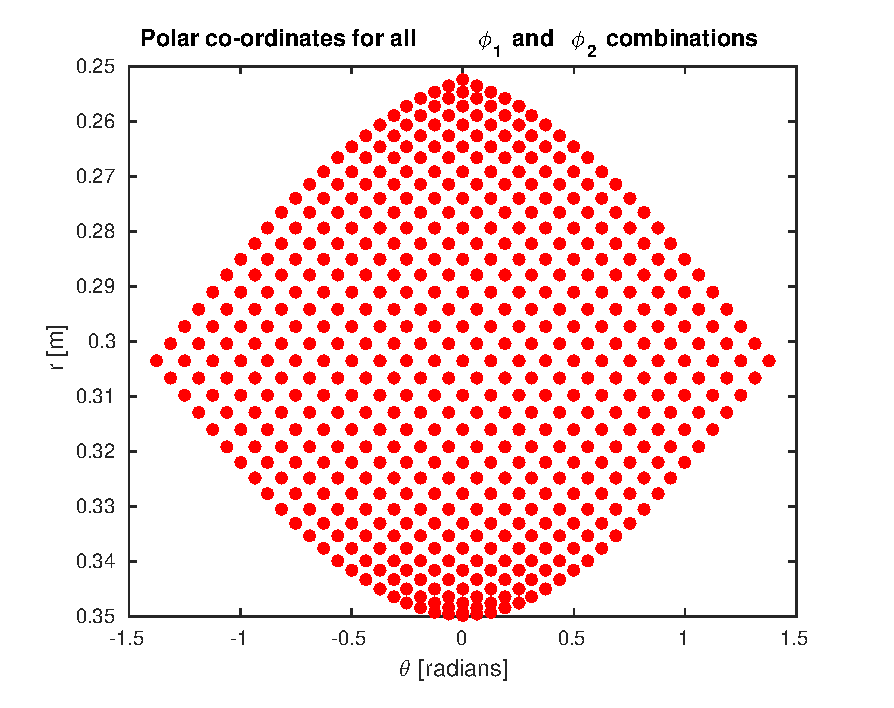
\includegraphics[width=0.8\textwidth]{images/geometry/forward-kinematic-leg-positions-5-30.eps}
\caption{Polar co-ordinates generated for all $\phi_1$ and $\phi_2$ combinations using forward kinematics: $l_1 = 5cm\ l_2 = 30cm$.}
\label{fig:Polar co-ordinates generated 5-30}
\end{figure}

\begin{figure}
\centering
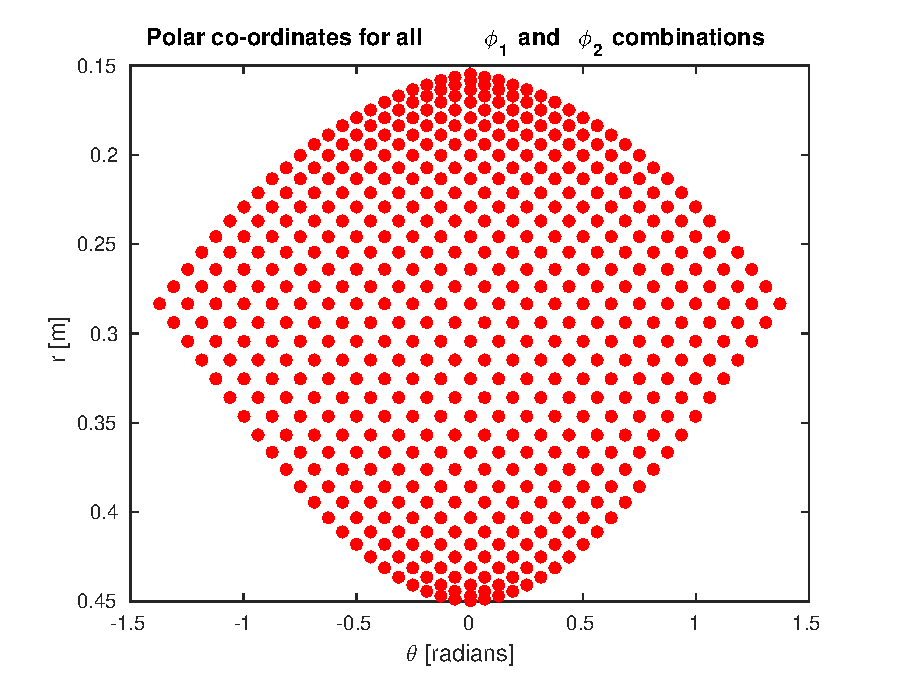
\includegraphics[width=0.8\textwidth]{images/geometry/forward-kinematic-leg-positions.eps}
\caption{Polar co-ordinates generated for all $\phi_1$ and $\phi_2$ combinations using forward kinematics: $l_1 = 15cm\ l_2 = 30cm$.}
\label{fig:Polar co-ordinates generated 15-30}
\end{figure}

\begin{figure}
\centering
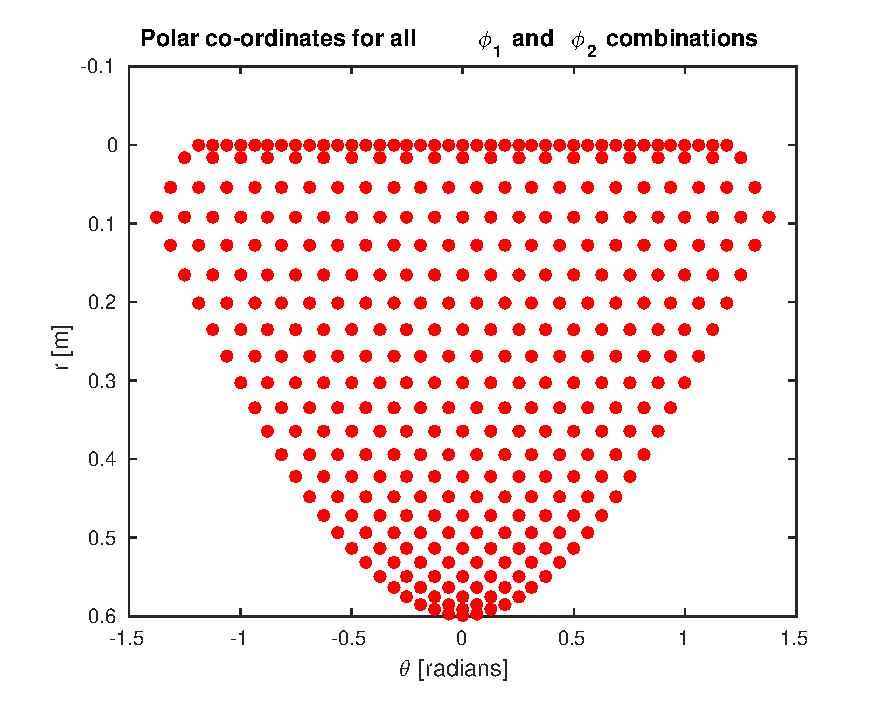
\includegraphics[width=0.8\textwidth]{images/geometry/forward-kinematic-leg-positions-30-30.eps}
\caption{Polar co-ordinates generated for all $\phi_1$ and $\phi_2$ combinations using forward kinematics: $l_1 = 30cm\ l_2 = 30cm$.}
\label{fig:Polar co-ordinates generated 30-30}
\end{figure}

\begin{figure}
\centering
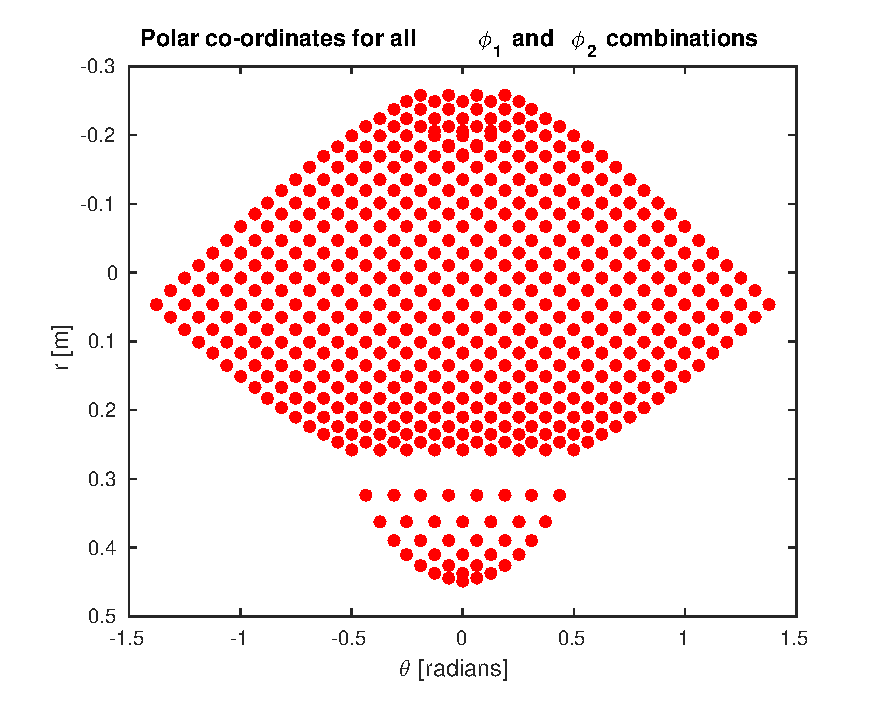
\includegraphics[width=0.8\textwidth]{images/geometry/forward-kinematic-leg-positions-30-15-complex.eps}
\caption{Polar co-ordinates generated for all $\phi_1$ and $\phi_2$ combinations using forward kinematics: $l_1 = 30cm\ l_2 = 15cm$.}
\label{fig:Polar co-ordinates generated 30-15}
\end{figure}

